\documentclass{article}
\usepackage{tikz}
\usetikzlibrary{arrows.meta}

\begin{document}

\begin{figure}[h]
    \centering
    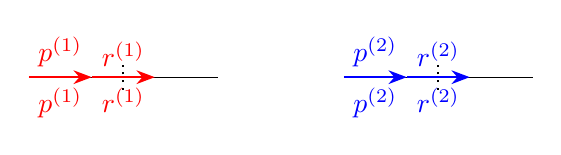
\begin{tikzpicture}[scale=0.8]

        % Define coordinates for the vertices
        \coordinate (A) at (0,0);
        \coordinate (B) at (1,0);
        \coordinate (C) at (2,0);
        \coordinate (D) at (3,0);
        \coordinate (E) at (4,0);
        \coordinate (F) at (5,0);
        \coordinate (G) at (6,0);
        \coordinate (H) at (7,0);
        \coordinate (I) at (8,0);

        % Draw the horizontal edges
        \draw[black] (A) -- (B);
        \draw[black] (F) -- (G);

        % Draw the vertical edges
        \draw[black] (B) -- (C);
        \draw[black] (C) -- (D);
        \draw[black] (H) -- (I);
        \draw[black] (G) -- (H);

        % Draw the red arrow in system 1
        \draw[red, thick, -Stealth] (A) -- (B) node[midway, below]{$p^{(1)}$} node[midway, above]{$p^{(1)}$};

        % Draw the blue arrow in system 2
        \draw[blue, thick, -Stealth] (F) -- (G) node[midway, below]{$p^{(2)}$} node[midway, above]{$p^{(2)}$};

        % Draw the red arrow in system 1
        \draw[red, thick, -Stealth] (B) -- (C) node[midway, below]{$r^{(1)}$} node[midway, above]{$r^{(1)}$};

        % Draw the blue arrow in system 2
        \draw[blue, thick, -Stealth] (G) -- (H) node[midway, below]{$r^{(2)}$} node[midway, above]{$r^{(2)}$};

        % Dotted lines
        \draw[dotted, black, thick] (1.5,-0.2) -- (1.5,0.2);
        \draw[dotted, black, thick] (6.5,-0.2) -- (6.5,0.2);

    \end{tikzpicture}
    \caption{Caption for the figure.}
    \label{fig:example}
\end{figure}

\end{document}